\section{Contexto}

El aprendizaje por refuerzo es una técnica del aprendizaje automático o \emph{Machine learning}, basada en cómo aprenden los seres vivos. Esta técnica de aprendizaje ha ganado mucha popularidad en los últimos años. Gran parte de esta popularidad se debe a los grandes avances que se han producido en últimas décadas. Una de las tecnologías que han aportado para este gran desarrollo viene de la mano de \textbf{\textit{OpenAI}} \cite {openia} con su librería "gym". Esta permite de manera simple entrenar algoritmos que jueguen y aprendan de un gran catálogo de juegos de la \textit{Atari 2600} entre muchos otros. 

Todos estos avances se ven además respaldados por grandes hazañas conseguidas en esta rama. Una de las primeras demostraciones se observa en 2015 con la victoria de \textbf{\textit{Alpha Go}} \cite {alphago}, la IA creada por \textit{Google}, contra un jugador profesional del videojuego \textit{Go} y posteriormente contra el 18 veces campeón del mundo del mismo juego. Más adelante, en 2017 \textit{DeepMind} \cite {deepmind} presentó \textbf{\textit{AlphaZero}}, una inteligencia artificial capaz de jugar a diversos juegos complejos como Ajedrez y Shogi. Lo más sorprendente era su capacidad de vencer a jugadores profesionales en estos juegos. Y finalmente uno de los últimos hitos conseguidos fue la creación de \textbf{\textit{AlphaStar}}, IA capaz de jugar a nivel profesional al videojuego de estrategia \textit{StarCraft II}. Una vez visto las capacidades de esta técnica de aprendizaje, explicaremos los conceptos que la forman.

\subsection{Definición de conceptos}

El aprendizaje por refuerzo consiste básicamente en la interacción que se produce entre un agente y su entorno al intentar conseguir un objetivo. Podemos usar la Figura \ref {fig:esquema_RL} como referencia para identificar los elementos básicos. Cuando un agente realiza una acción, esta produce una reacción también conocida como recompensa. Estas recompensas pueden ser positivas o negativas en función de si contribuyen o no la consecución del objetivo. A su vez, debido a la acción del agente, se produce un cambio en el entorno, hay un nuevo estado del entorno.

\begin{figure}[h]
	\centering
	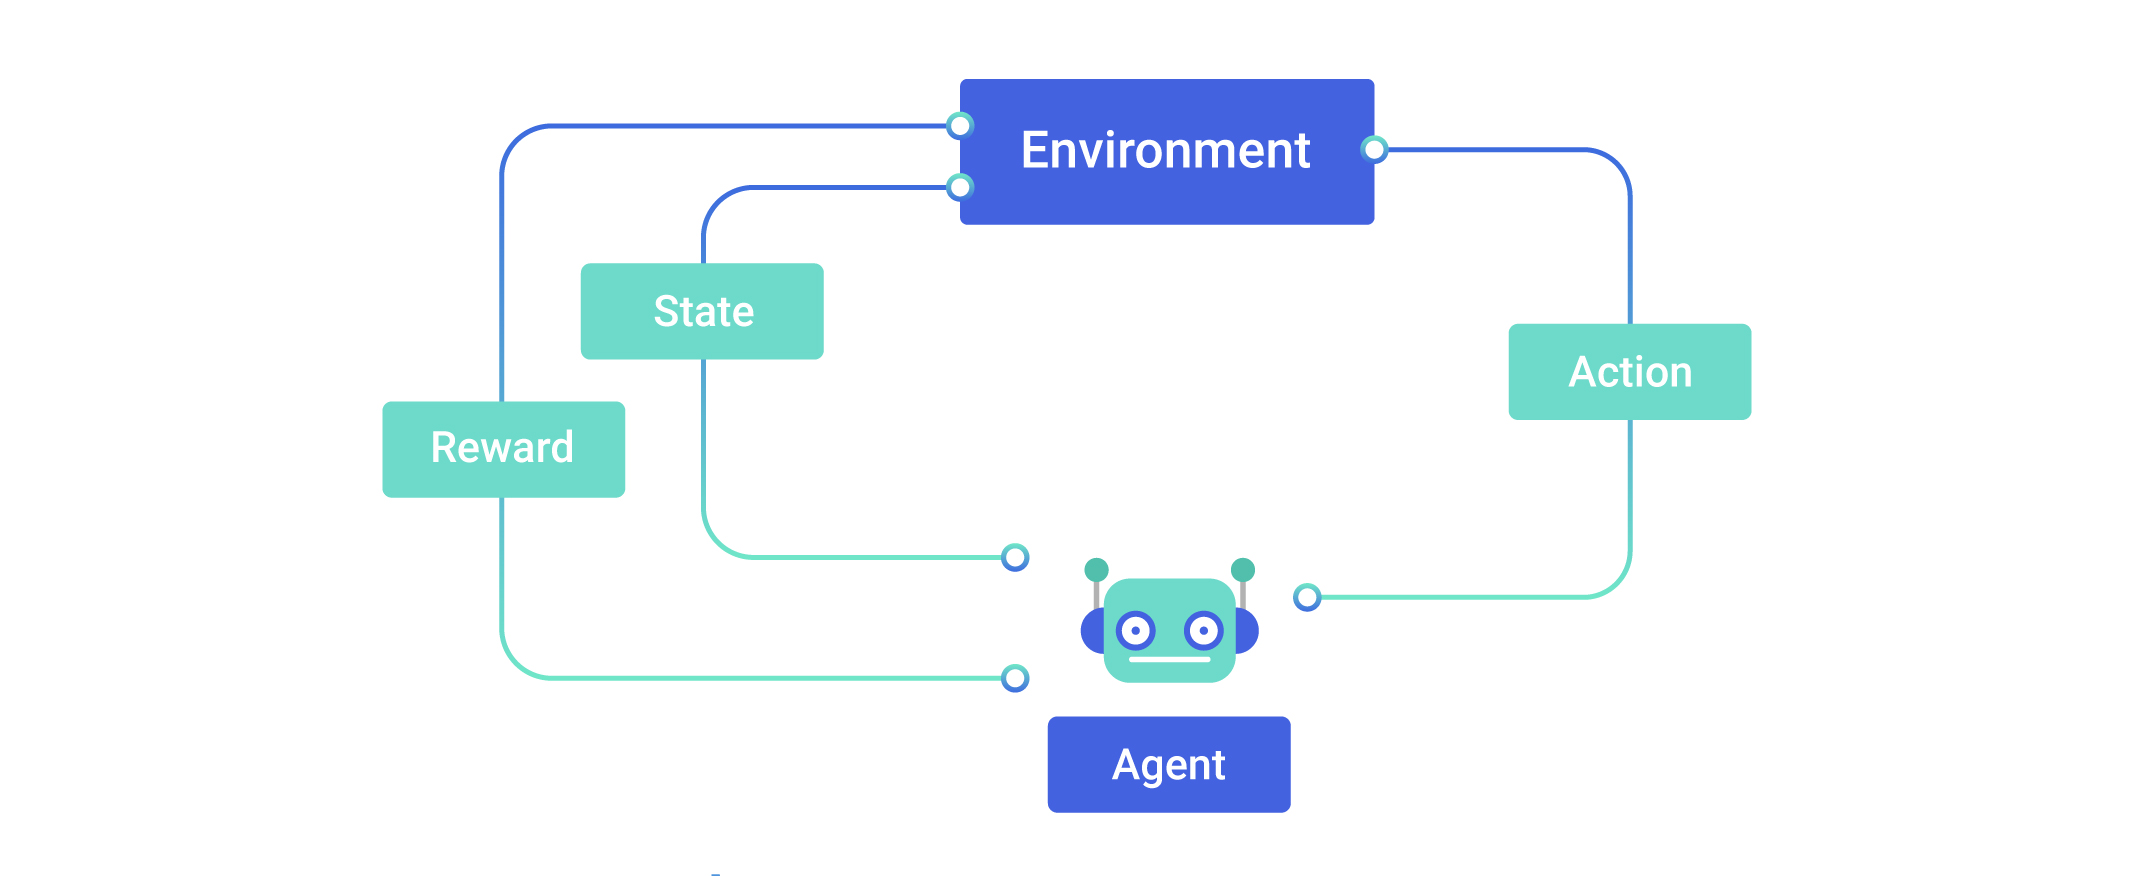
\includegraphics[width=0.7\textwidth]{img/esquema_RL.jpg}
	\caption{Esquema básico del aprendizaje por refuerzo \cite {RL_esquema}}
	\label{fig:esquema_RL}
\end{figure}

Para comprender mejor como se relaciona esto con la forma de aprender de los seres vivos usaremos un ejemplo de la naturaleza, este nos servirá para identificar los principales aspectos del aprendizaje por refuerzo. El contexto es un león que tiene como objetivo cazar a una presa. En esta situación, el agente sería el león y su objetivo consiste en cazar. Supongamos que se trata de un león joven que está aprendiendo a cazar, así que decide acercarse descuidadamente a la presa. Esto consistiría en la acción. Esta acción causa que la presa huya y se aleje del león. El nuevo estado es que la presa ha huido. Y además el agente ha recibido una recompensa negativa, puesto que su acción lo ha alejado de su objetivo. Gracias a esto, la criatura puede aprender que esta acción en este contexto no es apropiada. Después de diversas iteraciones en ese mismo entorno, este ser es capaz de aprender estrategias de a caza eficientes. Pero para aprender otra habilidad distinta, por ejemplo la defensa de un territorio, es necesario experimentar en otro entorno completamente distinto. De la misma forma pasa con las inteligencias artificiales, es necesario disponer de entornos diversos para poder investigar diferentes habilidades.  

De esta manera podemos definir los siguientes conceptos \cite {wiki_path}:
\begin{itemize}
	\item \textbf{Agente}: Cualquier ente capaz de realizar acciones. Usualmente un agente también tiene la capacidad de observar el estado de su entorno ya sea totalmente o de forma parcial.
	\item \textbf{Acciones}: Conjunto de posibles movimientos un agente puede realizar. En el contexto de la IA cabe destacar que los agentes normalmente solo pueden escoger acciones dentro de una lista discreta. Por ejemplo, en los videojuegos, las acciones suelen ser moverse en cualquier dirección, quedarse quieto, etc.
	\item \textbf{Entorno}: El mundo a través del cual el agente se mueve o actúa. Este responde y cambia en función a sus acciones. En concreto, en el contexto del aprendizaje por refuerzo, este toma el estado actual del agente y sus acciones como input y produce una recompensa y su nuevo estado.
	\item \textbf{Estado}: Situación concreta e inmediata en la cual se encuentra el agente. Si tratamos de un entorno tridimensional, consistiría en el lugar específico y el momento en el que se encuentra el agente, teniendo en cuenta su posición relativa a otros posibles elementos como obstáculos, enemigos, etc.
	\item \textbf{Recompensa}: Feedback por el cual medimos el éxito o el fracaso de las acciones de un agente en un estado determinado.  
\end{itemize}

Además, ahora solo estamos considerando un contexto de un solo agente. Esto aplicado a la inteligencia artificial se conoce como \emph{Single Agent Reinforcement Learning}. Esta rama dispone de una gran cantidad de entornos para poder entrenar inteligencias artificiales. El conjunto de entornos va desde más simples, como el mítico juego Pong donde el conjunto de acciones es muy limitado y la codificación del entorno es simple, hasta otros que permiten aprender comportamientos más complejos como invertir en bolsa.

\subsection{Descripción del problema}

En el apartado anterior hemos considerado solo entornos en los que se entrena un único agente, pero si hablamos de entornos para el entrenamiento de varios agentes, la realidad es muy distinta. La variedad de entornos se reduce drásticamente. En los próximos apartados profundizaremos más en las diferentes opciones de entornos disponibles. El problema que es que la mayoría de estos carecen de muchos aspectos que pueden ser interesantes para la investigación. Hablamos de aspectos relacionados con la comunicación entre agentes, relaciones de comercio, interacciones simbióticas donde cada uno tenga un rol específico y deban cooperar usando sus puntos fuertes, cualquier tipo de cooperación o competición entre agentes, etc. Este tipo de interacciones son interesantes, puesto que son básicas en los seres vivos. Volviendo con el ejemplo del león, si observamos los patrones de caza de estos animales cuando van en grupo, podemos observar que se comunican entre ellos y que cada uno tiene roles distintos que se complementan y cooperan entre sí. Y fijándonos en las interacciones humanas podemos encontrar infinidad de ejemplos del mismo tipo.

Por las razones mencionadas previamente, el problema que trataremos de solucionar es la \textbf{falta de entornos multiagente con características de complejas de interacción entre los agentes}, como comercio, comunicación directa, cooperación de diferentes roles, etc. Crear entornos complejos con estos aspectos de interacción puede aportar un gran beneficio a la humanidad, ya que se pueden descubrir métodos o técnicas útiles para resolver problemas de la vida real. Un ejemplo muy claro sería la coordinación de automóviles autónomos. Estos vehículos tendrán la capacidad de comunicarse para tomar decisiones que tendrán un impacto en el entorno. Entre mejor sea su estrategia de conducción y su coordinación entre ellos, será más sencillo que cumplan su objetivo. Y diferentes estrategias podrían conseguir resultados muy diferentes. Entrenar a estas inteligencias en entornos de un solo agente llevaría posiblemente a soluciones poco eficientes. Por ello es necesario investigar en la rama del \emph{Multi Agent Reinforcement Learning} (MARL), pero para poder hacerlo son necesarios entornos que implementen estas características. Y eso es precisamente lo que se realizará en este proyecto.

\subsection{Actores implicados}

Este trabajo de fin de grado se sitúa en el marco de la \emph{Facultad de Informática de Barcelona} (FIB) y más concretamente dentro del grupo de investigación \emph{High Performance Artificial Intelligence} (HPAI), que tiene como objetivo principal investigar y avanzar el estado del arte en técnicas de inteligencia artificial \cite{hpai} \cite{bsc-hpai}. Este equipo de investigación a su vez se sitúa en el marco del \emph{Barcelona Supercomputing Center - Centro Nacional de Supercomputación} (BSC-CNS), organización dedicada a la computación y conocida por albergar el supercomuputador \emph{MareNostrum}. El público objetivo que se beneficiará directamente de una solución para este problema es la comunidad dedicada al \emph{Reinforcement Learning} (RL) y más específicamente la comunidad de MARL. Del mismo modo, será esta comunidad la que principalmente usará esta solución. De forma indirecta, esta solución aportará beneficios a gran parte de la sociedad, ya que gracias a ella será posible la investigación de soluciones a problemas de áreas muy diversas, ya sea la conducción de automóviles autónomos, inteligencias artificiales para videojuegos, etc. 




